\subsection*{Hypothesis 3}

Reviews with higher book rating have higher helpfulness ratings.\\
\noindent
\textbf{Metric:} Correlation coefficient (e.g., Pearson's correlation) between review rating and helpfulness score.\\
\noindent
\textbf{Missing Values:}
\begin{itemize}
    \item \textit{`review/score`:} remove the entire sample
    \item \textit{`review/helpfulness`:} remove the entire sample
\end{itemize}
\noindent
\textbf{Data Transformation:}
\begin{itemize}
    \item \textit{`review/score`:} no operations required
    \item \textit{`review/helpfulness`:} $helpfulness = \frac{x}{y} \sqrt(y)$
\end{itemize}\vspace{0.5cm}
\noindent
\textbf{Description and Results}
As in the previous hypothesis, we decided to deal with missing values and data transformation directly with a MongoDB query. With the data ready to
be processed, we decided to perform a prior investigation on the distribution of votes on the 4 rating categories. As shown by Figure \ref{fig:h3_votes_distribution},
there is a \textbf{positive bias} as people are more prone to vote a positive reviews rather than a negative one. Specifically, the large majority of votes
for rating 5, were composed by a number of total votes just equal to 1. This introduces a bias in our results, since according to the formula used 
to compute the helpfulness score, such a small number of total votes would lead to a small helpfulness score.
To avoid this we decided to retain only the reviews with a number of total votes greater than 20.

\begin{figure}[H]
    \centering
    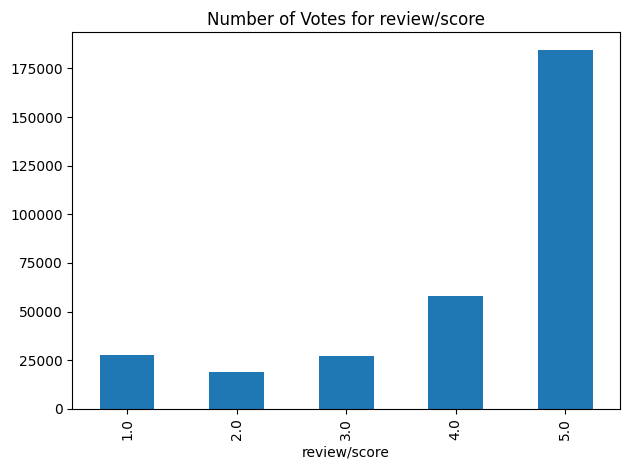
\includegraphics[width=0.5\textwidth]{./figures/h3_votes_distribution.png}
    \caption{Distribution of votes on the 4 rating categories}
    \label{fig:h3_votes_distribution}
\end{figure}
\noindent 
The Spearman correlation coefficient between the two variables is equal to $0.5247$, with a p-value of $0.0$. \\
\textbf{Conclusion:}
The hypothesis is confirmed as there is a positive and statistically significant correlation between the two variables. This result is confirmed by 
the boxplot in Figure \ref{fig:h3_boxplot}.

\begin{figure}[H]
    \centering
    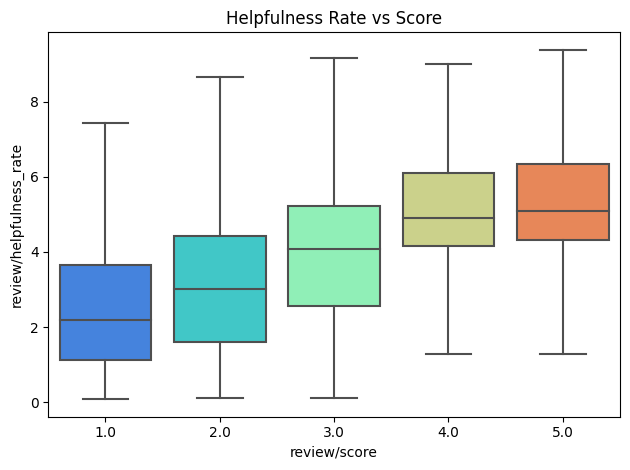
\includegraphics[width=0.5\textwidth]{./figures/h3_boxplot.png}
    \caption{Boxplot of the correlation between review rating and helpfulness score}
    \label{fig:h3_boxplot}
\end{figure}